\section{Kociemba's Optimal Solver}
\label{sec:kociemba}
Kociemba's optimal solver is an algorithm created with the purpose of finding the twist-wise optimal solution to any scrambled \rubik{}\cite{kociemba09} \cite{cubelovers92}. It has been developed by Herbert Kociemba who has studied physics and mathematics at Technische Universit�t Darmstadt\cite{TUD} (1974-1979) and is currently teaching at a gymnasium. His interest in the \rubik{} started in the 1980 and he implemented his first algorithm -- Kociemba's Two Phase algorithm -- in 1990. See appendix \ref{chap:emailCorrespondence} for the e-mail correspondence with Herbert Kociemba.

The Kociemba's optimal solver consists of two phases and is based on Kociemba's Two Phase algorithm. The first phase is based on a principle called relabeling, which will be defined at first. 

%In the following the Kociemba optimal solver will be described in detiail. Kociemba's Algorithm finds a solution to a scrambled \rubik{} using two phases and is based on another algorithm by Kociemba called Two Phase Algorithm. In order to fully understand kociemba's algorithm a process called relabeling must be defined at first.

\subsection{Relabeling}
The relabeling process  starts with choosing an up face with a corresponding down face. Then choosing a front face with a corresponding back face. Each \facelet{} with the color of the up or down face is marked with the letters ``UD''.  %Each edge \cpiece{} on the front and back where the \cpiece{} does not contain a ``UD'' sticker is marked with the letters ``FB''. 
Every edge \cpiece{} that is not labeled with "`UD"' is labeled with "`FB"' on the front and back face.
Figure \ref{fig:relabelClean} shows an example.
\begin{figure}[hb]
	\centering
		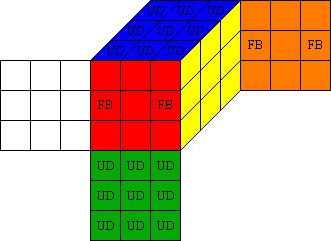
\includegraphics[scale = 0.8]{input/pics/relabelClean}
	\caption{\myCaption{A relabeled Rubik's Cube with the up and down faces as blue and green and red and orange as front and back.}}
	\label{fig:relabelClean}
\end{figure}
When relabeling a \rubik{} in the position $s$ it is written as $r(s)$. A \rubik{} in any position, $s$, is said to be in the set of positions called $H$(See subsection \ref{sub:theSubgroupH}) if and only if $r(s)=r(e)$.

\subsection{The subgroup $H$}
\label{sub:theSubgroupH}
%%% Beaware if the subgroup is introduced somewhere else. it should actually be. 
The moves U, U', U2, D, D', D2, R2, L2, F2 and B2 is the set of moves $A$. Using moves from $A$ on a position in $H$, will always result in a \rubik{} in $H$. The reason for this can easily be tested with a \rubik{}. If using one of the three up face moves or one of the three down face moves, the ``FB'' labels are not moved and the ``UD'' labels are simply rotated on the face that is being twisted, see figure \ref{fig:relabel2:D}. The last four moves are all very similar to each other. If any side face -- not up or down -- is \twist{}ed 180 degrees, the three \facelet{}s on the up face is moved to the down face and vice versa and thereby keeping all the ``UD'' labels on the up and down face and keeping the orientation correct. The two remaining relabeled \facelet{}s are swapped which keeps the ``FB'' labels placed and oriented correctly, see figure \ref{fig:relabel2:R2}.


\begin{figure}[!hb]
	\centering
	\subfloat[\myCaption{A relabeled cube that has been permutated with the move D.}]{\label{fig:relabel2:D}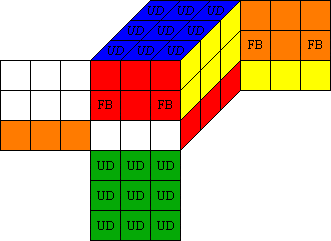
\includegraphics[width=0.45\textwidth]{input/pics/relabelD.PNG}}
	\hspace{0.05\textwidth}
	\subfloat[\myCaption{A relabeled cube that has been permutated with the move R2.}]{\label{fig:relabel2:R2}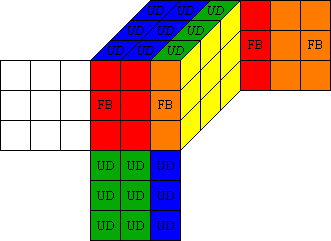
\includegraphics[width=0.45\textwidth]{input/pics/relabelR2.PNG}}
	\caption{\myCaption{Two positions which have been permuted with a move in $A$.}}
	\label{fig:relabel2}
\end{figure}
\subsection{Overall description}
\label{sub:overallDescription}
The first phase takes a scrambled cube $a$ and relabels it $r(a)$ then it finds a move sequence $b$ which will transform the relabeled cube into the subgroup $H$. This move will be denoted: $r(a)\cdot{}b \in H$. The second phase will then determine the length from the position $ab$ to the unit position $e$ by a table lookup. 


\begin{algorithm}[!h]                     
\caption{Kociemba's Algorithm \cite{rokicki09}}          
\label{alg:kociemba}        
\begin{algorithmic}[1]
\STATE $d=0$
\STATE {$l=\infty$}
\WHILE {$d<l$} 
	\FOR {$b \in S^{d}$}
		\IF {$r(ab) \in H$}
			\IF {$d + d_{2}(ab)<l$}
				\STATE {$l=d+d_{2}(ab)$}
			\ENDIF
		\ENDIF
	\ENDFOR
	\STATE {$d=d+1$}
\ENDWHILE
\STATE $b$ is now the optimal solution
\end{algorithmic}
\end{algorithm}

The search distance in the algorithm ($d$), see figure \ref{fig:searchExpansion} is initially set to zero and the total length ($l$) is set to infinite. The total length is the amount of moves used to get from $a$ to $e$, while $d$ is the limited search length to find a move sequence that transforms the \rubik{} into a position in $H$. 
The \textbf{while} loop will run as long as $d$ is less than $l$.
%For the first run this is true, and will only test if the scrambled \rubik{} already is in the subgroup $H$. If so it will continue since a solution that goes out of $H$ might be a faster solution. 

The \textbf{for} loop runs through all move sequences in the range $d$ -- recall that $S^d$ is the set containing every move sequence that uses $d$ twists. This search of moves in $S^d$ is called the first phase and is further described in \ref{sub:firstPhase}.
Then an \textbf{if}-statement checks if the move sequence transforms the cube into the subgroup $H$. If so the algorithm checks whether $d + d_2(ab)$ is less than the length of the last solution, if so, $d + d_2(ab)$ is the new shortest move sequence, $l$, to $e$. 
The lookup table denoted $d_2(ab)$ returns the numbers of twist required to transform a position in $H$ to the position $e$. This is done only by using moves in $A$. %$d_2(ab)$ is a lookup table which takes a position in $H$ and returns the number of twists it takes to transform the position to $e$ using moves in $A$ 
The lookup table is the second phase and is further described in the subsection \ref{sub:secondPhase}. 
The first time this \textbf{if}-statement is executed it will return true and this will be the new length of the solution. The \textbf{while} loop will end when $d$ is incremented to $l$. Figure \ref{fig:kociemba2} illustrates the algorithm.
\begin{figure}[htb]
	\centering
		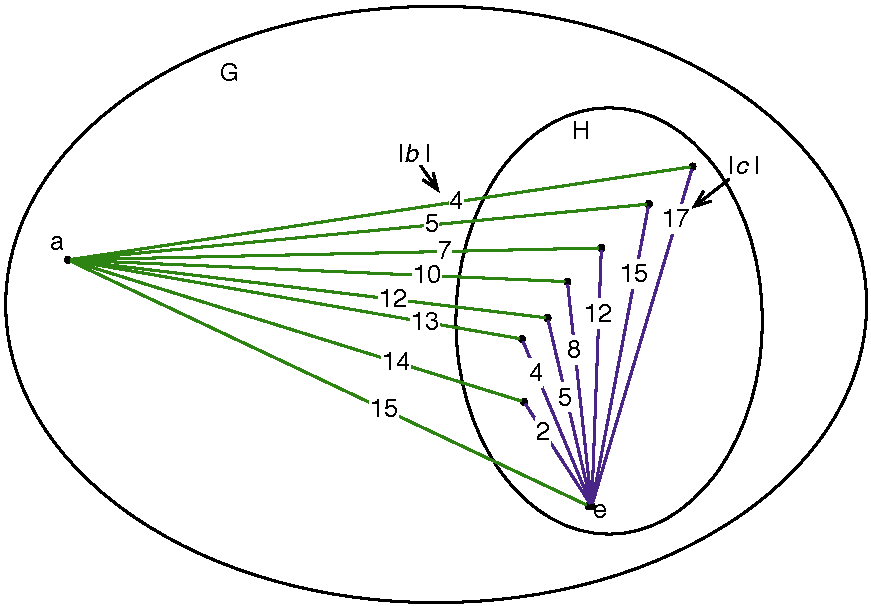
\includegraphics[scale=0.75]{input/pics/kocieambe2.pdf}
	\caption{\myCaption{ The lines going from $a$ to a point in $H$ is the move sequence denoted $b$. The lines from points in $H$ to the point $e$ is the move sequence denoted $c$ . The numbers beside the lines are the number of moves. Note that the moves in $c$ is decreasing as the numbers of moves in $b$ is increasing. The line that goes directly from $a$ to $e$ is the shortest move sequence possible. }}
	\label{fig:kociemba2}
\end{figure}

\subsection{First phase}
\label{sub:firstPhase}
The first phase finds a move sequence, $b$, from a position $a$ that transforms the \rubik{} into the subgroup $H$ this is done by going through all possible moves with a sequence of the length $d$. This is a breadth-first search algorithm \cite[pp. 729-731]{Rosen07}.
In figure \ref{fig:searchExpansion} the amount of elements in $S^d$ to a specific $d$ is illustrated.
An example of a search from a position $a$ is given. The algorithm starts by searching in $S^{d}$, where $d =  0$. This will give the position $a$ itself. The distance $d$ is then incremented to 1. This will result in 18 new possible move sequences all one twist away from $a$. Thereafter the $d$ is incremented and the search now moves 18 moves from the previous positions obtained in the search where $d = 1$. This allows a possibility for optimization of the algorithm since some of the moves will eventually be the same. e.g. the two move sequences R2 and R' R' is of length 1 and 2 respectively, but the result is the same transformed cube. The algorithm checks whether the transformed cube is in $H$ by relabeling it and checking if $r(ab) = r(e)$. The actual implementation of the algorithm may vary and will be omitted for now.

$d$ continues to be incremented until it reaches the length $l$. Since $l$ starts with the value infinite, it has to be changed in order to stop the loop. This happens in the second phase.

\begin{figure}[!hb]
	\centering
		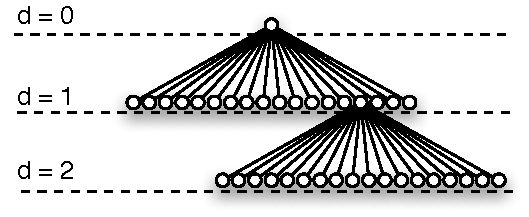
\includegraphics[scale=0.75]{input/pics/searchExpansion.pdf}
	\caption{\myCaption{As the distance of the search $d$ increases, the possible move sequences expands exponentially. For each vertex on the graph there is 18 child vertices. The amount of leaves for each search depth would be $18^{d}$.}}
	\label{fig:searchExpansion}
\end{figure}


\subsection{Second Phase}
\label{sub:secondPhase}
The goal of the second phase is to find the length of the shortest move sequence to transform the \rubik{} from a position in $H$ to $e$. A way to solve this problem is by having a lookup table. This table has to be very large, considering the amount of positions in $H$. 

The amount of positions can be calculated by imagining that one were to assemble the \rubik{}, starting with a disassembled \rubik{}. The first corner \cpiece{} can be placed in eight different places. The next corner has seven possible positions etc. Note that all \cpiece{}s in a cube in $H$ has the correct orientation. 
%until the last two corners which has a specific place since two corners can not be swapped. 
This gives $8! = 40320$ possibilities for the corners. 
The eight edges of the top and down layer can be placed similarly and also yields $8!$.  
The four edges of the middle layer can be placed in four different places this yield $4! = 24$. Since it is impossible to swap two corners without swapping any edges the amount of possibilities is halved. 
The final result is $\frac{4!\cdot(8!)^{2}}{2} \approx 19.508\cdot10^{9}$ elements in $H$.
The actual implementation of such a table will be discussed in section \emph{Remember reference here}. 